\documentclass[12pt, a4paper, oneside]{ctexart}
\usepackage{amsmath, amsthm, amssymb, bm, color, framed, graphicx, hyperref, mathrsfs}
\usepackage[inline]{enumitem}
\usepackage{tikz}

\title{\textbf{多元统计分析课程作业2}}
\author{Phlins}
\date{\today}
\linespread{1.5}
\definecolor{shadecolor}{RGB}{241, 241, 255}
\newcounter{problemname}
\newenvironment{problem}{\begin{shaded}\stepcounter{problemname}\par\noindent\textbf{题目\arabic{problemname}. }}{\end{shaded}\par}
\newenvironment{solution}{\par\noindent\textbf{解答. }}{\par}
\newenvironment{note}{\par\noindent\textbf{题目\arabic{problemname}的注记. }}{\par}

\begin{document}

\maketitle

\begin{problem}
4.2.
设一个二元正态总体有 $\mu_{1}=0, \mu_{2}=2, \sigma_{1 1}=2, \sigma_{2 2}=1$ 和 $\rho_{1 2}=0. \, 5.$  
\begin{enumerate}[label=(\alph*)]
    \item 写出二元正态密度
    \item 把广义平方距离的表达式 $\: ( \, x-\mu\, )^{\prime} \Sigma^{-1} \, ( \, x-\mu\, )$ )写成 $x_{1}$ 和 $x_{2}$ 的函数
    \item 确定含50\%概率的常密度轮廓线(并画出草图)
\end{enumerate}
\end{problem}

\begin{solution}
    \begin{enumerate}[label=(\alph*)]
        \item 已知:
        \begin{gather*}
            \because p=2,\mu=\begin{bmatrix}
                0\\
                2
            \end{bmatrix},\Sigma=\begin{bmatrix}
                2 & \frac{1}{\sqrt{2}}\\
                \frac{1}{\sqrt{2}} & 1
            \end{bmatrix}\\
            \therefore|\Sigma|=\frac{3}{2},\Sigma^{-1}=\begin{bmatrix}
                \frac{2}{\sqrt{3}} & -\frac{\sqrt{2}}{3}\\
                -\frac{\sqrt{2}}{3} & \frac{2}{\sqrt{3}} 
            \end{bmatrix}\\
            f(x)=\frac{1}{(2\pi)\sqrt{\frac{3}{2}}}\:\exp\left(-\frac{1}{2}\left[\:\frac{2}{3}x_{1}^{2}-\frac{2\sqrt{2}}{3}x_{1}(x_{2}-2)+\frac{4}{3}(x_{2}-2)^{2}\:\right]\right)
        \end{gather*}
        \item 
        $$\frac{2}{3}x_{1}^{2}-\frac{2\sqrt{2}}{3}x_{1}(x_{2}-2)+\frac{4}{3}(x_{2}-2\:)^{2}$$
        \item
        $c^{2}=\chi_{2}^{2}(0.5)=1.39.$ 中心位于$[0,2]$,长轴半径为$\sqrt{\lambda_1}c=\sqrt{2.366}\sqrt{1.39}=1.81$的椭圆。长轴方向为$e=\{0.888,0.460\}$。短轴方向为$e=\{-0.460,0.888\}$,短轴半径为$\sqrt{\lambda_{2}}c=\sqrt{0.634}\sqrt{1.39}=0.94$.
    \end{enumerate}
\end{solution}

\begin{note}
    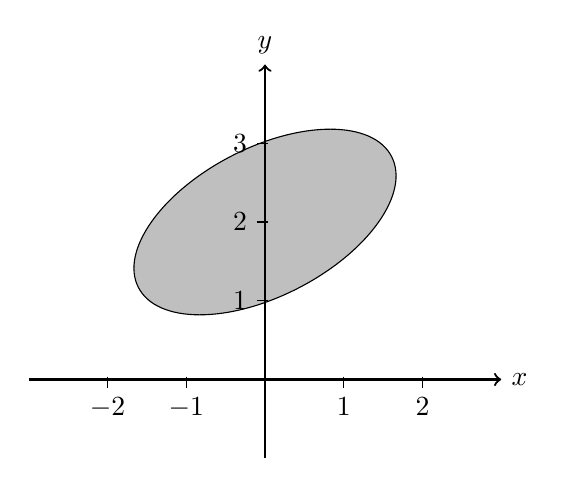
\begin{tikzpicture}
        \begin{scope}[rotate around={27.38:(0,2)}]
            \draw[fill=gray!50] (0,2) ellipse (1.81cm and 0.94cm);
        \end{scope}
        
        % 画出坐标轴
        \draw[thick,->] (-3,0) -- (3,0) node[right] {$x$};
        \draw[thick,->] (0,-1) -- (0,4) node[above] {$y$};

        % 在x轴上添加标签
        \foreach \x in {-2,-1,1,2} {
            \draw (\x,1pt) -- (\x,-3pt) node[anchor=north] {$\x$};
        }

        % 在y轴上添加标签
        \foreach \y in {1,2,3} {
            \draw (1pt,\y) -- (-3pt,\y) node[anchor=east] {$\y$};
        }

        % 旋转的角度为arctan(0.460/0.888),大约为27.38度

    \end{tikzpicture}
\end{note}

\begin{problem}
4.3. 设 $\boldsymbol{X}$ 服从$\mu^{\prime}=[-3,1,4]$和
$$
\boldsymbol{\Sigma}=\begin{bmatrix} {{1}} & {{-2}} & {{0}} \\ {{-2}} & {{5}} & {{0}} \\ {{0}} & {{0}} & {{2}} \end{bmatrix} 
$$
的 $N_{3}(\mu,\Sigma)$ ,下列各对随机变量中哪几数对相互独立?请解释
\begin{enumerate}[label=(\alph*)]
    \item  $X_{1}$ 和 $X_{2}$ 
    \item  $X_{2}$ 和 $X_{3}$ 
    \item $(X_{1}, X_{2})$ 和 $X_{3}$ 
    \item $\frac{X_{1}+X_{2}} {2}$ 和 $X_{3}$ 
    \item $X_{2}$ 和 $X_{2}-\frac{5} {2} X_{1}-X_{3}$ 
\end{enumerate}
\end{problem}

\begin{solution}
    根据结果 4.5,我们将零协方差与统计独立性联系起来:
    \begin{enumerate}[label=(\alph*)]
        \item 不,$\sigma_{12}\neq0$   
        \item 是的,$\sigma_{23}=0$
        \item 是的,$\sigma_{13}=\sigma_{23}=0$
        \item 是的,根据结果 4.3,$(x_1+x_2)/2$ 和 $x_{3}$ 是联合正态的,它们的协方差是 $\frac{1}{2}\sigma_{13}+\frac{1}{2}\sigma_{23}=0$
        \item 不,根据结果 4.3,取$A=\begin{bmatrix}0&1&0\\-\frac{5}{2}&1&-1\end{bmatrix}$,计算$A\Sigma A^{\prime}$,可以看出协方差为10而不是0。
    \end{enumerate}
\end{solution}

\begin{problem}
    4.16
    设 $X_{1}, X_{2}, X_{3}$ 和 ${X}_{4}$ 是独立 $N_{p} (\mu,\Sigma)$ 随机向量
    \begin{enumerate}[label=(\alph*)]
        \item 对以下两个随机向量求边缘分布
        \begin{gather*}
V_{1}={\frac{1} {4}} X_{1}-{\frac{1} {4}} X_{2}+{\frac{1} {4}} X_{3}-{\frac{1} {4}} X_{4} \\
 V_{2}={\frac{1} {4}} X_{1}+{\frac{1} {4}} X_{2}-{\frac{1} {4}} X_{3}-{\frac{1} {4}} X_{4}
\end{gather*}
        \item 求(a)中定义的随机向量 $\mathbf{V}_{1}$ 和 $\mathbf{V}_{2}$ 的联合密度
    \end{enumerate}
\end{problem}
\newpage
\begin{solution}
    \begin{enumerate}[label=(\alph*)]
        \item 根据结果 4.8,取$c_1= c_3= 1/4, \quad c_2= c_4= - 1/4$ 和 $\mu_j= \mu$ ($j=1,...,4$),我们有 $\sum _{j= 1}^4c_j\mu_j= 0$ 和 $( \sum _{j= 1}^4c_j^2) \Sigma= \frac 14\Sigma$。因此,$V_1$ 是 $N(0,\frac14\Sigma)$。类似地,取$b_1=b_2=1/4$ 和 $b_3=b_4=-1/4$,我们发现 $V_{2}$ 是 $N(0,\frac{1}{4}\Sigma)$。
        \item 再次根据结果 4.8,我们知道 $V_{1}$ 和 $V_{2}$ 是联合多元正态分布,其协方差为
            $$
            (\sum_{j=1}^{4}b_{j}c_{j})\Sigma=\left(\frac{1}{4}(\frac{1}{4})+\frac{-1}{4}(\frac{1}{4})+\frac{1}{4}(\frac{-1}{4})+\frac{-1}{4}(\frac{-1}{4})\right)\Sigma=0
            $$
        即
        \begin{gather*}
            \begin{bmatrix}
                V_{1}\\
                V_{2}
            \end{bmatrix}
            \text{服从}
            N_{2p}\left(0,\begin{bmatrix}{\frac{1}{4}\Sigma}&{0}\\{0}&{\frac{1}{4}\Sigma}\end{bmatrix}\right)
        \end{gather*}
        所以 $2p$ 变量的联合密度为
        \begin{align*}
            f(v_{1}, v_{2})&=\frac{1}{(2\pi)^{p}|\frac{1}{4}\Sigma|}\exp\begin{bmatrix}{-\frac{1}{2}}[v_{1}^{\prime}, v_{2}^{\prime}]\begin{bmatrix}{\frac{1}{4}\Sigma}&{0}\\{0}&{\frac{1}{4}\Sigma}\end{bmatrix}^{-1}\begin{bmatrix}{v_{1}}\\{v_{2}}\end{bmatrix}\end{bmatrix}.\\
                            &=\frac{1}{(2\pi)^{p}|\frac{1}{4}\Sigma|}\exp\left(2(v_{1}^{\prime}\Sigma^{-1}v_{1}+v_{2}^{\prime}\Sigma^{-1}v_{2})\right)
        \end{align*}
    \end{enumerate}
\end{solution}

\begin{problem}
    4.18.
    试根据来自二维正态总体的随机样本
$$
X=\begin{bmatrix} {3} & {6} \\ {4} & {4} \\ {5} & {7} \\ {4} & {7} \\ \end{bmatrix} 
$$
求 $2 \times1$ 均值向量$\mu$和 $2 \times2$ 协方差矩阵$\Sigma$的极大似然估计
\end{problem}

\begin{solution}
    根据 4.11 结果, $\mu$ 和 $\Sigma$ 的最大似然估计分别为 $\hat{\mu}=\bar{x}=[4,6]^{\prime}$
    \begin{align*}
        \frac{1}{n}\sum_{j=1}^{n}\left(x_{j}-\bar{x}\right)\left(x_{j}-\bar{x}\right)^{\prime} &= \frac{1}{4} 
        \left\{
            \left(\begin{bmatrix}3\\6\end{bmatrix}-\begin{bmatrix}4\\6\end{bmatrix}\right)\left(\begin{bmatrix}3\\6\end{bmatrix}-\begin{bmatrix}4\\6\end{bmatrix}\right)^{\prime}+
            \left(\begin{bmatrix}4\\4\end{bmatrix}-\begin{bmatrix}4\\6\end{bmatrix}\right)\left(\begin{bmatrix}4\\4\end{bmatrix}-\begin{bmatrix}4\\6\end{bmatrix}\right)^{\prime}\right.\\
        &\left.+\left(\begin{bmatrix}5\\7\end{bmatrix}-\begin{bmatrix}4\\6\end{bmatrix}\right)\left(\begin{bmatrix}5\\7\end{bmatrix}-\begin{bmatrix}4\\6\end{bmatrix}\right)^{\prime}+
            \left(\begin{bmatrix}4\\7\end{bmatrix}-\begin{bmatrix}4\\6\end{bmatrix}\right)\left(\begin{bmatrix}4\\7\end{bmatrix}-\begin{bmatrix}4\\6\end{bmatrix}\right)^{\prime}
        \right\}\\
            &=\frac{1}{4}
            \left(\begin{bmatrix}-1\\0\end{bmatrix}\begin{bmatrix}-1&0\end{bmatrix}+\begin{bmatrix}0\\-2\end{bmatrix}\begin{bmatrix}0&-2\end{bmatrix}+\begin{bmatrix}1\\1\end{bmatrix}\begin{bmatrix}1&1\end{bmatrix}+\begin{bmatrix}0\\1\end{bmatrix}\begin{bmatrix}0&1\end{bmatrix}\right)\\
        &=\frac{1}{4}\begin{bmatrix}{2}&{1}\\{1}&{6}\end{bmatrix}
    \end{align*}
\end{solution}

\end{document}